\section{Aufgabenbeschreibung}

In der zunehmden digitalisierten Welt entstehen in jeglichen Bereichen immer mehr Daten, die eine Verarbeitung erfordern. Dies betrifft auch den Bereich des Einzelhandels, in dem Einkaufsdaten aus Kassenbons (s. Abbildung \ref{bon}) durch Big Data und BI-Technologien für die Auswertung in einen Kontext gebracht werden können. Daraus können Erkenntnisse über das Einkaufsverhalten der Kunden geschlossen werden, die als Entscheidungsgrundlage dienen können. In diesem Projekt wird dargestellt, wie eine solche Auswertung durchgeführt werden kann und welche Erkenntnisse daraus geschlossen werden können.

\begin{wrapfigure}[20]{l}{0.5\textwidth} %this figure will be at the right
  \centering
  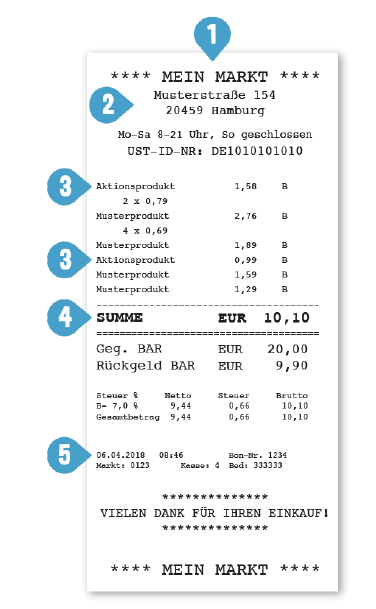
\includegraphics[width=0.5\textwidth]{kassenbon}
  \caption{Kassenbon (Quelle: DBIS-Aufgaben)}
  \label{bon}
\end{wrapfigure}

\noindent Der Kassenbon enhält die Bereiche (1) Filiale, (2) Standort, (3) Bonpositionen mit Verkaufspreisen, (4) die Summe der Verkaufspreise sowie (5) Datum, Kasse, Bedingung etc.
Der Fachbereich beschreibt die Abteilung, zu der die Produkte zugeordnet werden.

\begin{itemize}
  \itemsep0em
  \item Bonnummer
  \item Filiale
  \item Fachbereich/Fachabteilung
  \item Warengruppe
  \item Artikelnummer
  \item Produktbezeichnung
  \item Handelsmarke
  \item Trockensortiment (Ja, Nein)
  \item Verkaufsdatum mit Uhrzeit
  \item Verkaufsmenge
  \item Verkaufspreis
  \item Aktionsware (optional)
  \item Rabattierte Ware(optional)
\end{itemize}

\newpage




